\section{Luminosity functions}
One of the most effective methods for quantifying galaxy evolution over cosmic time is with the luminosity function (\gls{lf}). Luminosity functions are statistical distributions that describe the spatial density of astronomical objects at various luminosities and redshifts, and so are a fundamental tool for quantifying their evolution across cosmic time \citep{han_evolution_2012, dai_mid-infrared_2009, wylezalek_galaxy_2014}. In this section, I focus on and give a review of \gls{ir} \gls{lf}s and provide a brief overview of other wavelengths. In \cref{Sec: Luminosity Functions Chapter}, I will introduce how to calculate \gls{lf}s and show the results of preliminary tests. 

\subsection{Malmquist Bias}

\Cref{Fig: ZFOURGE Distribution} illustrates the relationship between luminosity and redshift for all sources in \gls{zfourge} \citep{straatman_fourstar_2016}. A prominent feature is the presence of Malmquist bias \citep{malmquist_relations_1922}, a selection effect whereby the most distant objects are also among the brightest observed. This bias arises from the operational characteristics of telescopes. When observations are conducted, telescopes are pointed at a specific region in space and data is collected over a predetermined exposure time. For an astronomical object to be detected by any given telescope, it must meet a minimum threshold of brightness or distance. This is known as the flux limit and is defined by the quantity of energy received by the area of a telescope's mirrors over a specified duration (measured in $J \ m^{-2} \ s^{-1}$). This measurement can be influenced by a variety of factors, including, but not limited to, thermal conditions.

\begin{figure}[h]
    \centering
    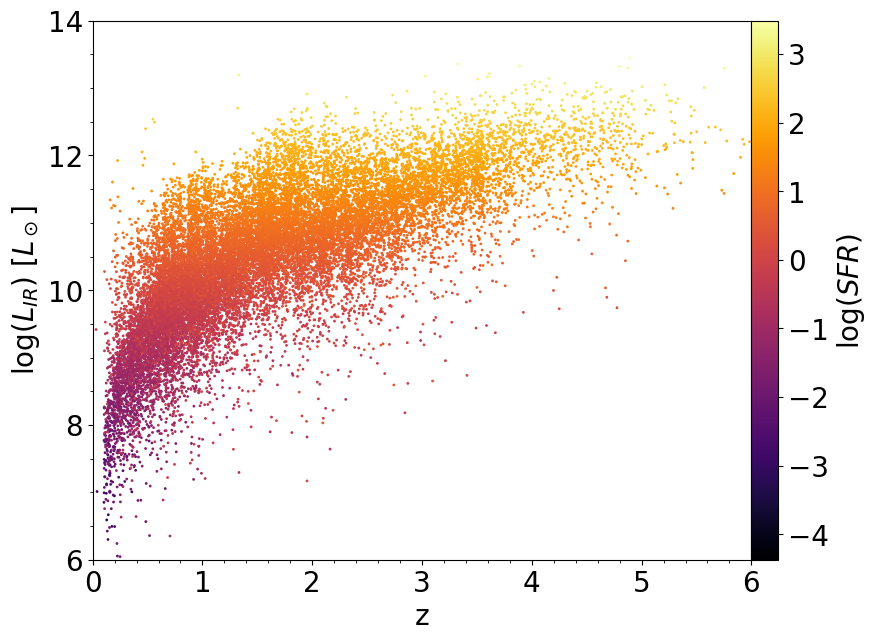
\includegraphics[width=\textwidth]{Figures/ZFOURGE Initial Distribution.png}
    \caption{Distribution of ZFOURGE galaxies used in this analysis.}
    \label{Fig: ZFOURGE Distribution}
\end{figure}

Galaxies under the ``main curve" of \cref{Fig: ZFOURGE Distribution} still exist, but are outside the detection threshold of (in this case) the Spitzer Space Telescope. To observe the most distant and faint objects, it is essential to develop more sensitive telescopes, such as the recently operational \gls{jwst} \citep{gardner_james_2006} which offers unprecedented sensitivity and resolving power in the \gls{ir} \citep{labiano_wavelength_2021}. Additionally, the Square Kilometer Array \citep{dewdney_square_2009} represents a next-generation radio telescope capable of identifying high-redshift radio galaxies through their neutral hydrogen content, the most prevalent element in the extremely early universe \citep{furlanetto_cosmology_2006}.

By studying the simple distribution of galaxies --- the number of galaxies per unit volume of space through cosmic time --- we are able to observe how the \gls{lss} of the universe has changed and begin to understand how various types of galaxies have influenced that evolution. The most direct method of measuring the distribution of galaxies is with the \gls{lf}. The effect of Malmquist bias is effectively minimised in \gls{lf}s because number density corrects for the difference in the volume over which galaxies of different luminosities are observable. By expressing the count of galaxies as a function of volume and luminosity, it provides a more accurate representation of the intrinsic galaxy population. How this is achieved in practice is explained in \cref{Sec: Luminosity Functions Chapter}.